\documentclass{beamer}
\usepackage{amsmath}
\usepackage{amssymb}
\usepackage{amsfonts}
\usepackage{bm}

\usepackage{graphicx}
\usepackage{tikz}
\graphicspath{{./code/figures/}}
\usepackage{hyperref}
\hypersetup{
  colorlinks=true,
  linkcolor=blue,
  filecolor=magenta,
  urlcolor=blue,
}

\usepackage{tikz}
\usepackage{pgfplots}
\pgfplotsset{compat=1.18}

\usetheme{Boadilla}
\usecolortheme{seahorse}

\title{Bayesian Logistic Regression}
\author{Vasilis Gkolemis}
\institute{ATHENA RC | HUA}
\date{June 2025}

\begin{document}

% Automatically insert agenda slide at the start of each section
\AtBeginSection[]{
  \begin{frame}{Program}
    \tableofcontents[currentsection]
  \end{frame}
}


\begin{frame}
  \titlepage
  \vfill
  \footnotesize
  \textcopyright\
  Vasilis Gkolemis, 2025. Licensed under CC BY 4.0.
\end{frame}


% Slide 1: Introduction
\begin{frame}{Logistic Regression as a Probabilistic Model}
\begin{itemize}
  \item In binary classification, we model the probability of label $y \in \{0,1\}$ given input $\mathbf{x} \in \mathbb{R}^d$:
  \[
    p(y = 1 \mid \mathbf{x}, \mathbf{w}) = \sigma(\mathbf{w}^\top \mathbf{x})
  \]
  \item $\sigma(z) = \frac{1}{1 + e^{-z}}$ is the logistic sigmoid function.
  \item In a Bayesian setting, we place a prior over $\mathbf{w}$ and infer the posterior:
  \[
    p(\mathbf{w} \mid \mathcal{D}) \propto p(\mathbf{w}) \prod_{n=1}^{N} p(y_n \mid \mathbf{x}_n, \mathbf{w})
  \]
\end{itemize}
\end{frame}

% Slide 2: Posterior Challenges
\begin{frame}{Why Approximate Inference?}
\begin{itemize}
  \item The posterior is not analytically tractable due to the non-conjugate likelihood.
  \item The logistic sigmoid does not lead to a conjugate posterior with a Gaussian prior.
  \item Approximate inference methods are needed:
  \begin{itemize}
    \item Laplace Approximation
    \item Importance Sampling
    \item Markov Chain Monte Carlo (MCMC)
  \end{itemize}
\end{itemize}
\end{frame}

% Slide 3: The Toy Example
\begin{frame}{2D Toy Example}
\begin{itemize}
  \item We create a small dataset with $N=50$ samples:
  \begin{itemize}
    \item $\mathbf{x}_n \in [-3, 3]^2$, $y_n \sim \mathrm{Bernoulli}(\sigma(\mathbf{w}^\top \mathbf{x}_n))$, where $\mathbf{w}^\star = (0.5, -0.6)$
  \end{itemize}
  \item Classes are slightly overlapping to reflect realistic uncertainty.
\end{itemize}

\vspace{0.5em}
\begin{center}
  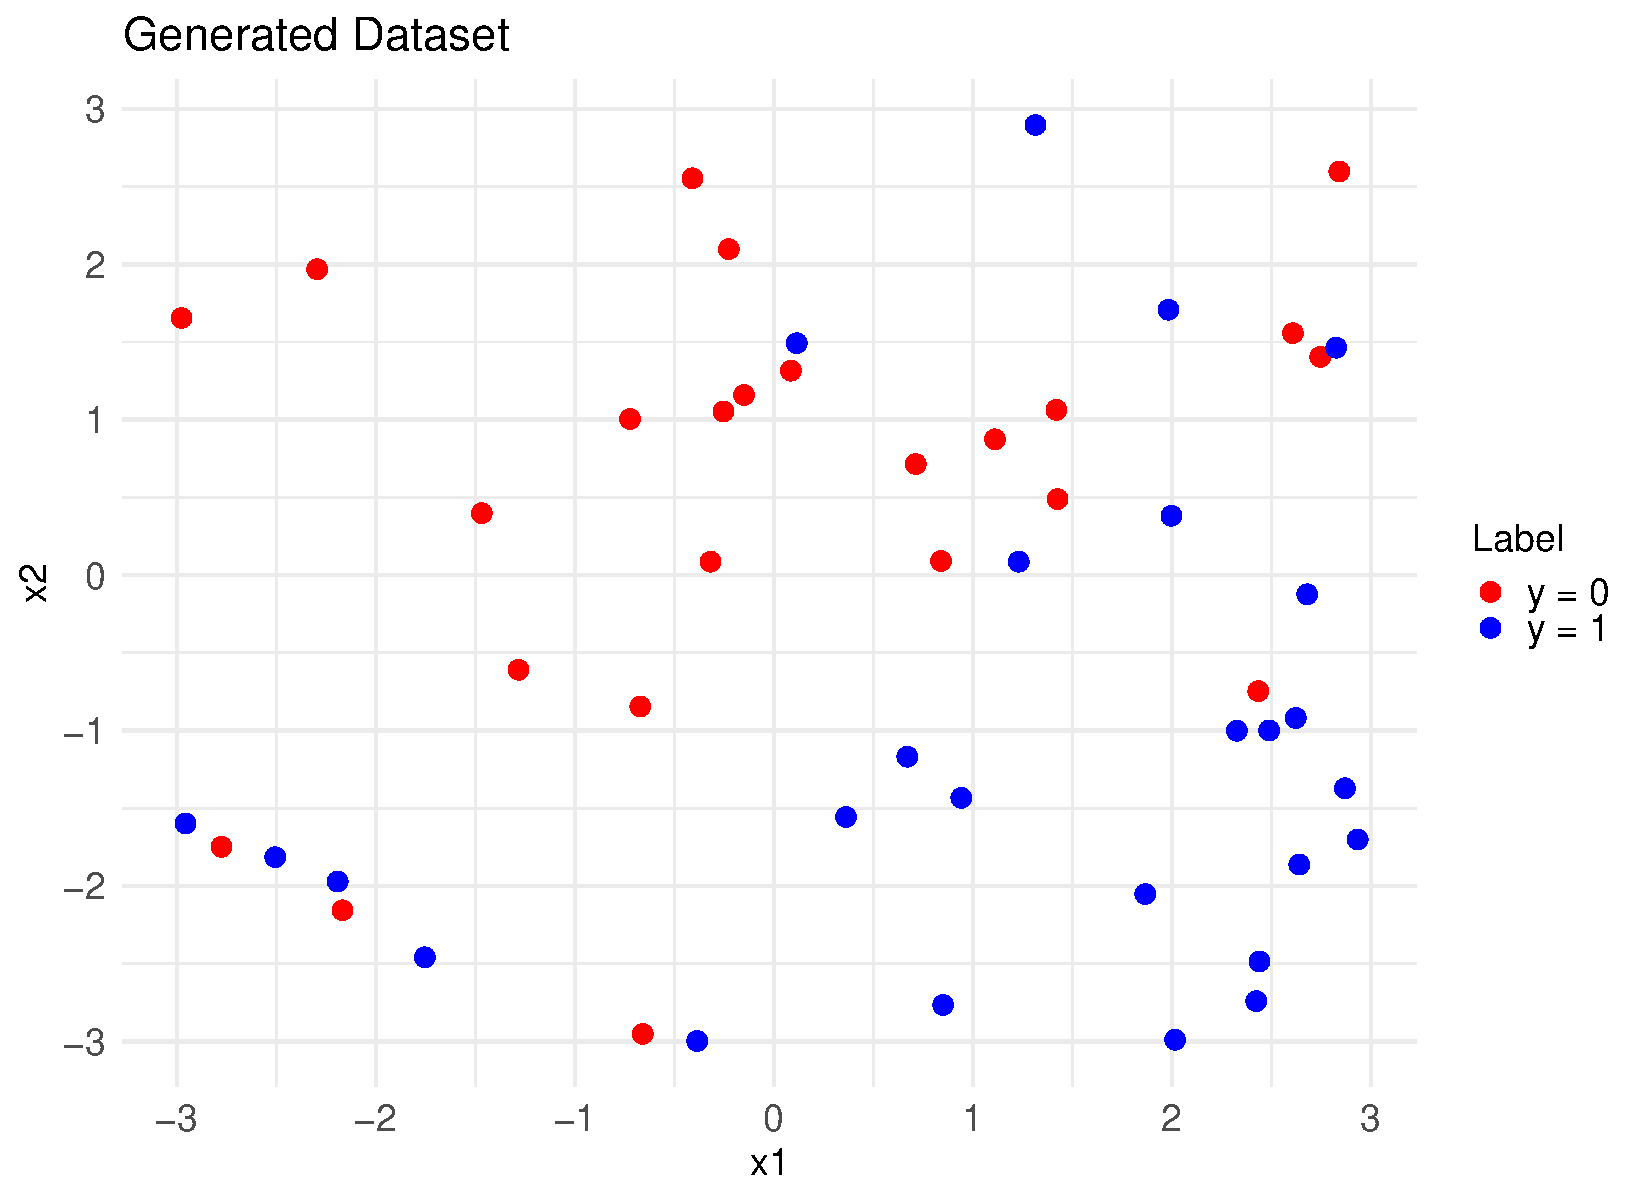
\includegraphics[width=0.6\linewidth]{generated_dataset.pdf}
\end{center}
\end{frame}

% Slide 4: Model Summary
\begin{frame}{Model Specification}
\begin{itemize}
  \item Prior over weights:
  \[
    \mathbf{w} \sim \mathcal{N}(\mathbf{0}, \alpha^{-1} \mathbf{I})
  \]
  \item Likelihood:
  \[
    p(\mathcal{D} \mid \mathbf{w}) = \prod_{n=1}^{N} \sigma(\mathbf{w}^\top \mathbf{x}_n)^{y_n} (1 - \sigma(\mathbf{w}^\top \mathbf{x}_n))^{1 - y_n}
  \]
  \item Posterior:
  \[
    p(\mathbf{w} \mid \mathcal{D}) \propto p(\mathbf{w}) p(\mathcal{D} \mid \mathbf{w}) \quad \text{(approximated)}
  \]
\end{itemize}
\end{frame}

\section{Laplace Approximation}

% Slide 3: Laplace idea
\begin{frame}{Laplace Approximation: Idea}
  \begin{itemize}
  \item Is it reasonable to approximate the posterior with a Gaussian?
  \item Yes:
    \begin{itemize}
    \item It is an incremental improvement over MAP
    \item Many ML methods rely on a single configuration; Laplace is a natural extension
    \item When the posterior is dominated by a single mode
      \end{itemize}
  \item No:
    \begin{itemize}
    \item When the posterior is multimodal or highly skewed
    \item Unfortunately, this is often the case in practice
    \end{itemize}
\end{itemize}

\[
p(\boldsymbol{\theta} \mid \mathcal{D}) \approx \mathcal{N}(\bm{\theta}; \bm{\mu}, \bm{\Sigma}), \quad \text{where:} \quad
\]
\begin{itemize}
    \item[] \(\bm{\mu} = \) MAP estimate (mode of posterior), often denoted as \(\hat{\boldsymbol{\theta}}\)
    \item[] \(\bm{\Sigma} = \) inverse Hessian of the log posterior at the mode, denoted as \(\mathbf{H}^{-1}\)
\end{itemize}
\end{frame}

\begin{frame}{Laplace Approximation: How it Works}
  \[p(\boldsymbol{\theta} \mid \mathcal{D}) \approx \mathcal{N}(\bm{\theta}; \bm{\mu} = \hat{\boldsymbol{\theta}}, \bm{\Sigma}=\mathbf{H}^{-1})\]
  \begin{itemize}
  \item Why setting $\bm{\mu}$ to $\hat{\boldsymbol{\theta}}$, i.e., the MAP estimate?
  \item $p(\bm{\theta} \mid \mathcal{D})$ is proportional to the product of the prior and likelihood:
    Search for the point that maximizes $L(\boldsymbol{\theta})p(\boldsymbol{\theta}) \Rightarrow$ MAP estimate
  \item[]
    \[
      \hat{\boldsymbol{\theta}} = \arg\max_{\boldsymbol{\theta}} \log p(\boldsymbol{\theta} \mid \mathcal{D}) = \arg\max_{\boldsymbol{\theta}} \left( \log p(\boldsymbol{\theta}) + \sum_{i=1}^N \log p(y_i \mid \mathbf{x}_i, \boldsymbol{\theta}) \right)
    \]
  \item It is a simple optimization problem:
    \begin{itemize}
    \item Use gradient-based methods (e.g., Newton-Raphson, L-BFGS)
    \item Can easily solve high-dimensional problems, if autograd is available
    \end{itemize}
\end{itemize}
\end{frame}

\begin{frame}{Laplace Approximation: How it Works}
  \[p(\boldsymbol{\theta} \mid \mathcal{D}) \approx \mathcal{N}(\bm{\theta}; \bm{\mu} = \hat{\boldsymbol{\theta}}, \bm{\Sigma}=\mathbf{H}^{-1})\]
  \begin{itemize}
  \item Why setting \(\bm{\Sigma}\) to \(\mathbf{H}^{-1}\), i.e., the inverse Hessian?
  \item The MAP is a turning point. What happens there?
    \begin{itemize}
    \item Imagine it as a mountain peak in the log-posterior landscape
    \item The gradient vanishes:
      \(\nabla \log p(\boldsymbol{\theta} \mid \mathcal{D})\big|_{\boldsymbol{\theta} = \hat{\boldsymbol{\theta}}} = 0\
      \)
    \item The Hessian captures local curvature:
      \(\mathbf{H} = -\nabla^2 \log p(\boldsymbol{\theta} \mid \mathcal{D})\big|_{\boldsymbol{\theta} = \hat{\boldsymbol{\theta}}}\)
    \end{itemize}
  \item \(\mathbf{H} \in \mathbb{R}^{d \times d}\) (where \(d\) is the number of parameters), where:
    \[\mathbf{H}_{ij} = -\frac{\partial^2 \log p(\boldsymbol{\theta} \mid \mathcal{D})}{\partial \theta_i \partial \theta_j}\bigg|_{\boldsymbol{\theta} = \hat{\boldsymbol{\theta}}}\]
    \item \(\bm{\Sigma} = \mathbf{H}^{-1}\):
    \begin{itemize}
  \item High curvature (large values in \(\mathbf{H}\)) means steep slope, low uncertainty
  \item Low curvature (small values in \(\mathbf{H}\)) means flat slope, high uncertainty
    \end{itemize}

    \end{itemize}
\end{frame}

% Slide 4: Derivation via Taylor expansion
\begin{frame}{Taylor Expansion and Laplace Approximation}
  \begin{itemize}
  \item Taylor expansion approximates a function \(f(\boldsymbol{\theta})\) around a point \(\hat{\boldsymbol{\theta}}\) with a polynomial, i.e., a smooth curve:
    \[
      f(\boldsymbol{\theta}) \approx f(\hat{\boldsymbol{\theta}}) + \nabla f(\hat{\boldsymbol{\theta}})^\top (\boldsymbol{\theta} - \hat{\boldsymbol{\theta}}) + \frac{1}{2} (\boldsymbol{\theta} - \hat{\boldsymbol{\theta}})^\top \nabla^2 f(\hat{\boldsymbol{\theta}}) (\boldsymbol{\theta} - \hat{\boldsymbol{\theta}})
    \]
  \item a second-order Taylor expansion around the MAP estimate is:
\[
\log p(\boldsymbol{\theta} \mid \mathcal{D}) \approx \log p(\hat{\boldsymbol{\theta}} \mid \mathcal{D})
- \frac{1}{2} (\boldsymbol{\theta} - \hat{\boldsymbol{\theta}})^\top \mathbf{H} (\boldsymbol{\theta} - \hat{\boldsymbol{\theta}})
\]
where \(\mathbf{H} = -\nabla^2 \log p(\boldsymbol{\theta} \mid \mathcal{D}) \big|_{\hat{\boldsymbol{\theta}}}\) is the (negative) Hessian at the mode.

\item Exponentiating both sides gives the Laplace approximation of the posterior:
\[
p(\boldsymbol{\theta} \mid \mathcal{D}) \approx \mathcal{N}(\boldsymbol{\theta}; \hat{\boldsymbol{\theta}}, \mathbf{H}^{-1})
\]
\end{itemize}
\end{frame}

\begin{frame}{Laplace Approximation: Summary}
So the Laplace Approximation gives:
\[
p(\boldsymbol{\theta} \mid \mathcal{D}) \approx \mathcal{N}(\bm{\theta}; \bm{\mu}=\hat{\bm{\theta}}, \bm{\Sigma}=\mathbf{H}^{-1})\]

\begin{itemize}
\item Computational considerations:
\begin{itemize}
\item MAP estimate \(\hat{\boldsymbol{\theta}}\) is a point estimate, not a distribution
\item If gradients are available, it is efficient to compute
\item Hessian \(\mathbf{H}\) is computed at the MAP estimate
\item Up to \(O(d^3)\) for inversion, where \(d\) is the number of parameters
  \item Cannot work for very high-dimensional problems (e.g., \(d > 1000\))
\end{itemize}
\item Final conclusion:

  \textit{Laplace Approximation is easy to implement and compute but may be inaccurate if the posterior is multimodal or skewed.}
\end{itemize}
\end{frame}


\begin{frame}{Why Laplace Works in Logistic Regression}

Consider Bayesian logistic regression:
\[
p(\boldsymbol{\theta} \mid \mathcal{D}) \propto p(\mathcal{D} \mid \boldsymbol{\theta}) \cdot p(\boldsymbol{\theta})
\]

\medskip

\begin{itemize}
  \item \textbf{Likelihood:} \(p(\mathcal{D} \mid \boldsymbol{\theta}) = \prod_{n} \sigma(\boldsymbol{\theta}^\top \mathbf{x}_n)^{y_n}(1 - \sigma(\boldsymbol{\theta}^\top \mathbf{x}_n))^{1 - y_n}\)
  \item \textbf{Prior:} \(p(\boldsymbol{\theta}) = \mathcal{N}(\boldsymbol{\theta}; \mathbf{0}, \tau^2 \mathbf{I})\)
\end{itemize}

\medskip

\[
\Rightarrow p(\boldsymbol{\theta} \mid \mathcal{D}) = \text{Gaussian prior} \cdot \prod_n \text{sigmoid likelihood}
\]

\medskip

\textbf{Conclusion:} The posterior is a Gaussian (prior) where each sigmoid slices off a portion of the mass. The resulting distribution has a single mode, making Laplace a good approximation.

\end{frame}

\begin{frame}{Laplace Approximation in our Toy Example}

\begin{center}
  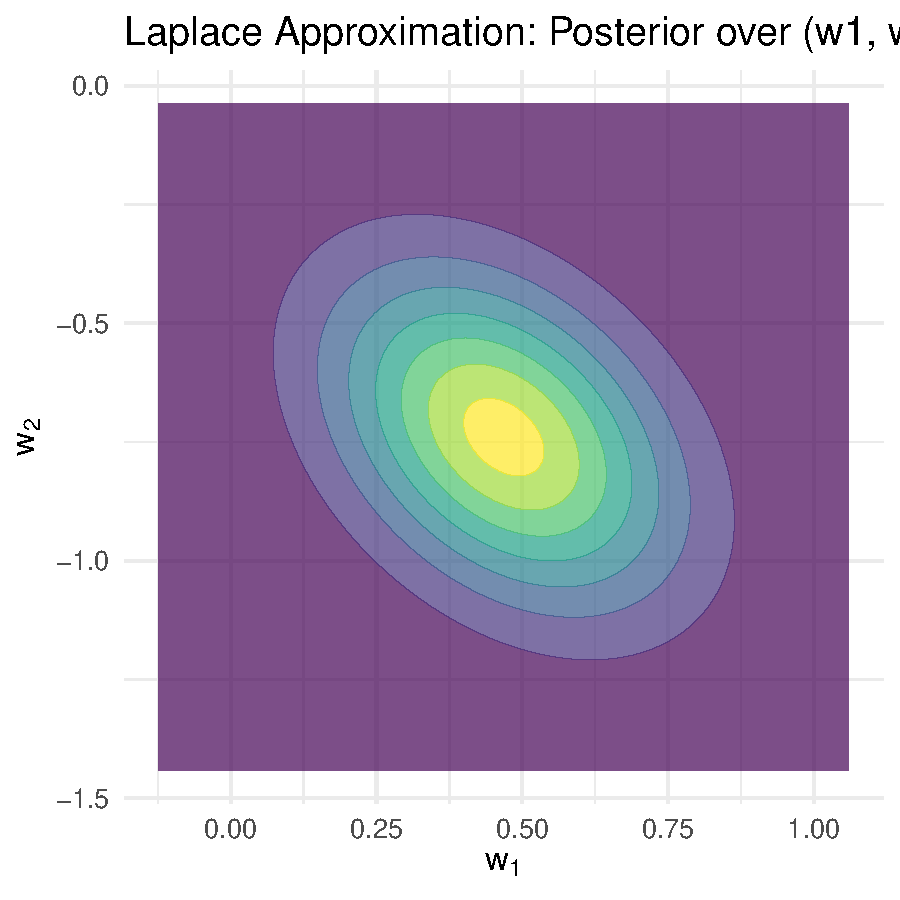
\includegraphics[width=0.6\linewidth]{laplace_posterior_contours.pdf}
\end{center}

\end{frame}



\begin{frame}{Laplace Approximation in our Toy Example}

\begin{center}
  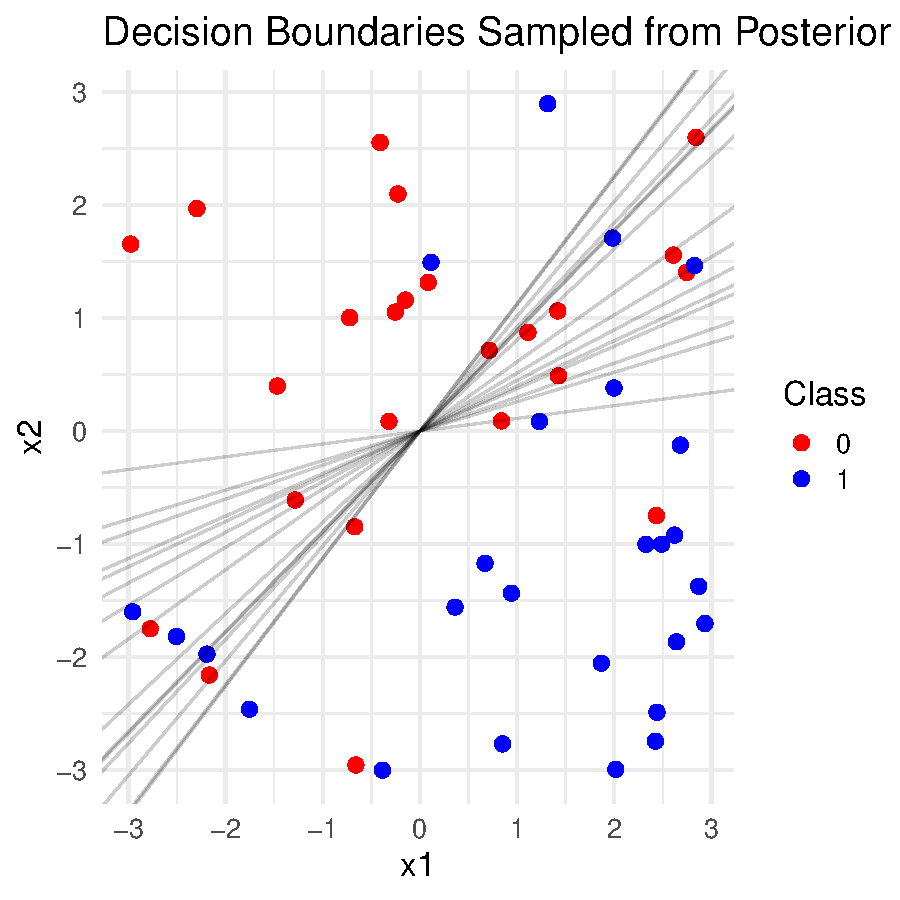
\includegraphics[width=0.6\linewidth]{laplace_decision_boundaries.pdf}
\end{center}

\end{frame}

\section{Importance Sampling}
\begin{frame}{Importance Sampling: Motivation}
\begin{itemize}
    \item Goal: Compute expectations under a difficult distribution \( p(\theta) \) (e.g., posterior).
    \item Direct sampling from \( p(\theta) \) is hard or impossible.
    \item Instead, sample from a simpler proposal distribution \( q(\theta) \).
\end{itemize}
\[
\mathbb{E}_{p}[f(\theta)] = \int f(\theta) p(\theta) d\theta \quad \text{but} \quad p(\theta) \text{ is hard to sample from}.
\]
\end{frame}

\begin{frame}{Importance Sampling Estimator}
\[
\mathbb{E}_{p}[f(\theta)] = \int f(\theta) \frac{p(\theta)}{q(\theta)} q(\theta) d\theta = \mathbb{E}_{q}\left[f(\theta) w(\theta)\right]
\]
where the \alert{importance weights} are
\[
w(\theta) = \frac{p(\theta)}{q(\theta)}.
\]
\end{frame}

\begin{frame}{Practical Importance Sampling}
Given samples \(\{\theta_i\}_{i=1}^N \sim q(\theta)\):
\[
\hat{\mu} = \frac{\sum_{i=1}^N w_i f(\theta_i)}{\sum_{i=1}^N w_i}, \quad \text{where} \quad w_i = \frac{p(\theta_i)}{q(\theta_i)}.
\]
\begin{itemize}
    \item Weights are normalized to sum to 1.
    \item Effective when \( q(\theta) \) covers \( p(\theta) \) well.
\end{itemize}
\end{frame}

\begin{frame}{Importance Sampling in Bayesian Inference}
\begin{itemize}
    \item Target posterior: \( p(\theta | X, y) \propto p(y | X, \theta) p(\theta) \).
    \item Proposal \( q(\theta) \) can be prior or Laplace approximation.
    \item Importance weights:
\[
w_i = \frac{p(y | X, \theta_i) p(\theta_i)}{q(\theta_i)}.
\]
    \item Samples \(\theta_i \sim q(\theta)\) weighted to approximate the posterior.
\end{itemize}
\end{frame}

\begin{frame}{Importance Sampling with Prior Proposal}
\begin{columns}
  \column{0.5\textwidth}
  \centering
  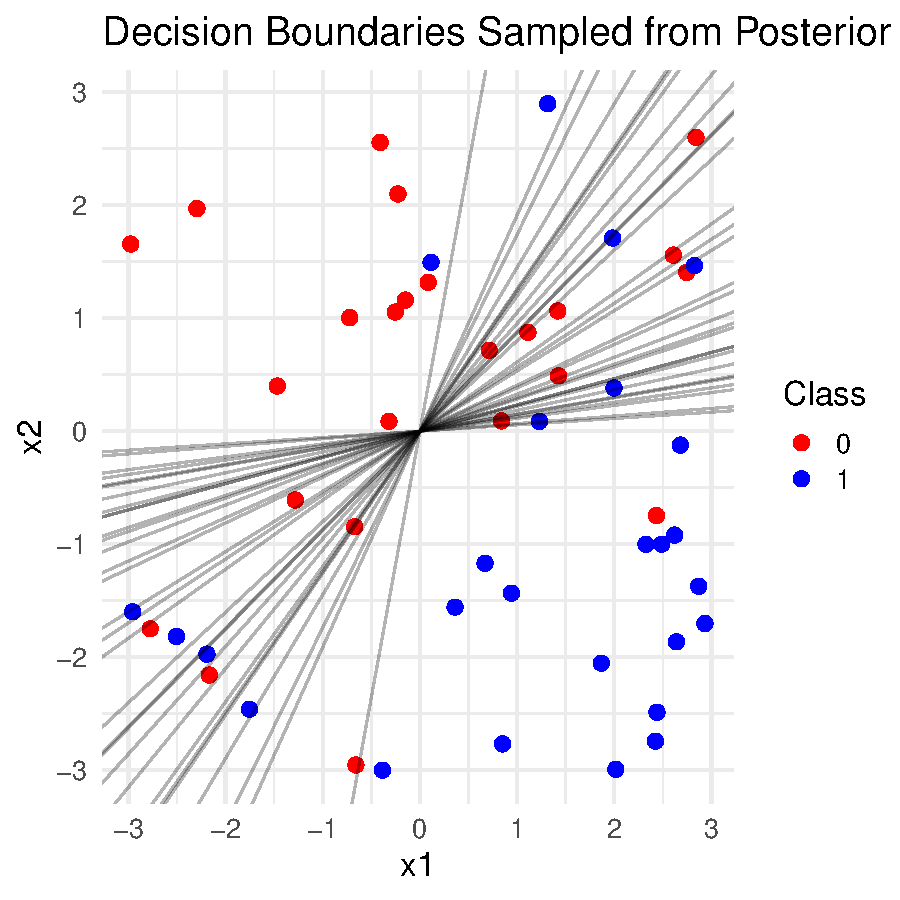
\includegraphics[width=\textwidth]{importance_sampling_from_prior.pdf}

  \column{0.5\textwidth}
  \small
  \begin{itemize}
    \item Proposal distribution \( q(\theta) = p(\theta) \) (prior).
    \item Samples drawn directly from prior.
    \item Importance weights correct for data likelihood.
    \item May have high variance if prior poorly matches posterior.
  \end{itemize}
\end{columns}
\end{frame}

\begin{frame}{Importance Sampling with Laplace Approximation Proposal}
\begin{columns}
  \column{0.5\textwidth}
  \centering
  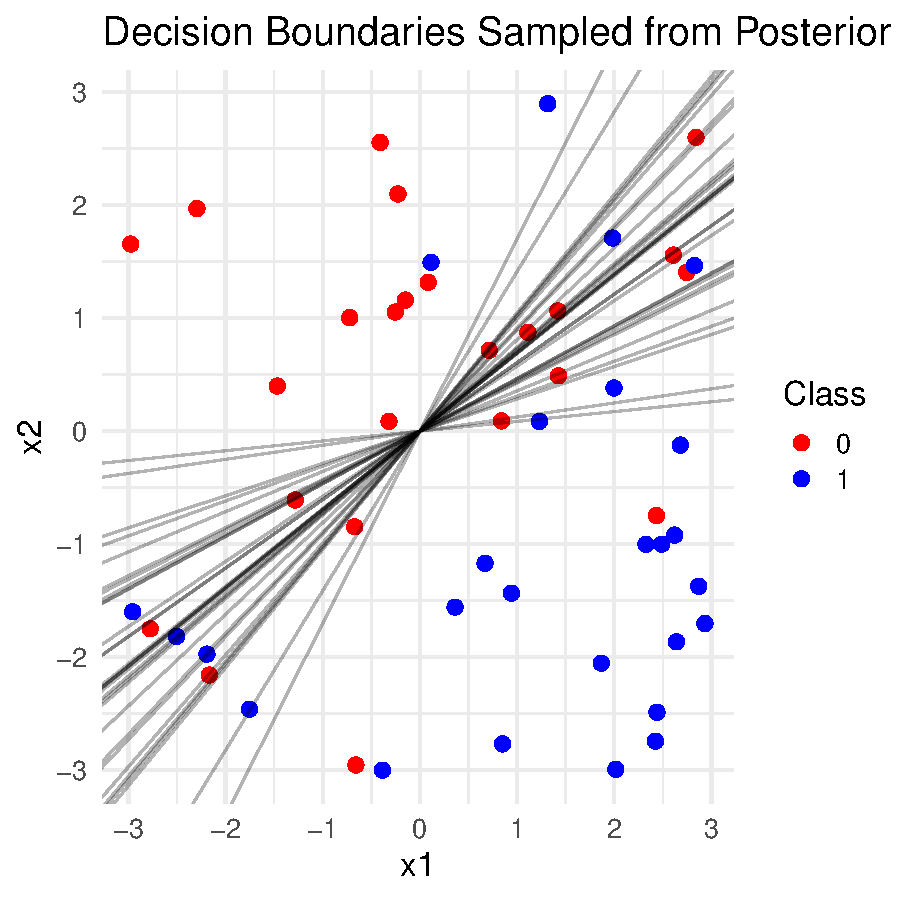
\includegraphics[width=\textwidth]{importance_sampling_from_laplace.pdf}

  \column{0.5\textwidth}
  \small
  \begin{itemize}
    \item Proposal distribution \( q(\theta) \approx \mathcal{N}(\hat{\theta}, H^{-1}) \) (Laplace approx).
    \item Samples concentrated near MAP estimate.
    \item Importance weights reweight samples to correct approximation.
    \item Typically lower variance than prior proposal.
  \end{itemize}
\end{columns}
\end{frame}

\section{MCMC}

\begin{frame}{Markov Chain Monte Carlo (MCMC) for Bayesian Inference}
\begin{itemize}
  \item Goal: Sample from posterior distribution \(p(\theta \mid X, y)\) when direct sampling is difficult.
  \item Construct a Markov chain whose stationary distribution is the posterior.
  \item Generates dependent samples that approximate the posterior as the chain runs.
  \item Widely applicable to complex models where exact inference is intractable.
\end{itemize}
\end{frame}

\begin{frame}{Metropolis-Hastings Algorithm}
\begin{itemize}
  \item Start from an initial parameter \(\theta^{(0)}\).
  \item At step \(t\), propose \(\theta^*\) from proposal distribution \(q(\theta^* \mid \theta^{(t-1)})\).
  \item Calculate acceptance probability:
  \[
    \alpha = \min\left(1, \frac{p(\theta^* \mid X,y) q(\theta^{(t-1)} \mid \theta^*)}{p(\theta^{(t-1)} \mid X,y) q(\theta^* \mid \theta^{(t-1)})}\right)
  \]
  \item Accept \(\theta^*\) with probability \(\alpha\), else keep \(\theta^{(t-1)}\).
  \item Ensures the chain converges to posterior distribution.
\end{itemize}
\end{frame}

\begin{frame}{MCMC for Bayesian Logistic Regression}
\begin{itemize}
  \item Posterior \(p(\theta \mid X,y) \propto p(y \mid X,\theta) p(\theta)\) is non-conjugate.
  \item MCMC provides a way to approximate the posterior without analytic form.
  \item Samples \(\{\theta^{(t)}\}_{t=1}^T\) can be used for:
  \begin{itemize}
    \item Estimating expectations (posterior means, variances).
    \item Predictive distributions.
    \item Visualizing uncertainty, e.g. decision boundary variation.
  \end{itemize}
\end{itemize}
\end{frame}

\begin{frame}{Practical Considerations}
\begin{itemize}
  \item \textbf{Burn-in}: Discard initial samples until chain stabilizes.
  \item \textbf{Thinning}: Keep every \(k\)-th sample to reduce autocorrelation.
  \item \textbf{Tuning}: Proposal distribution parameters (e.g., step size) affect acceptance rate and mixing.
  \item Diagnostics needed to check convergence (trace plots, effective sample size).
\end{itemize}
\end{frame}

\begin{frame}{MCMC Samples: Decision Boundaries from Posterior}
  \begin{figure}
    \centering
    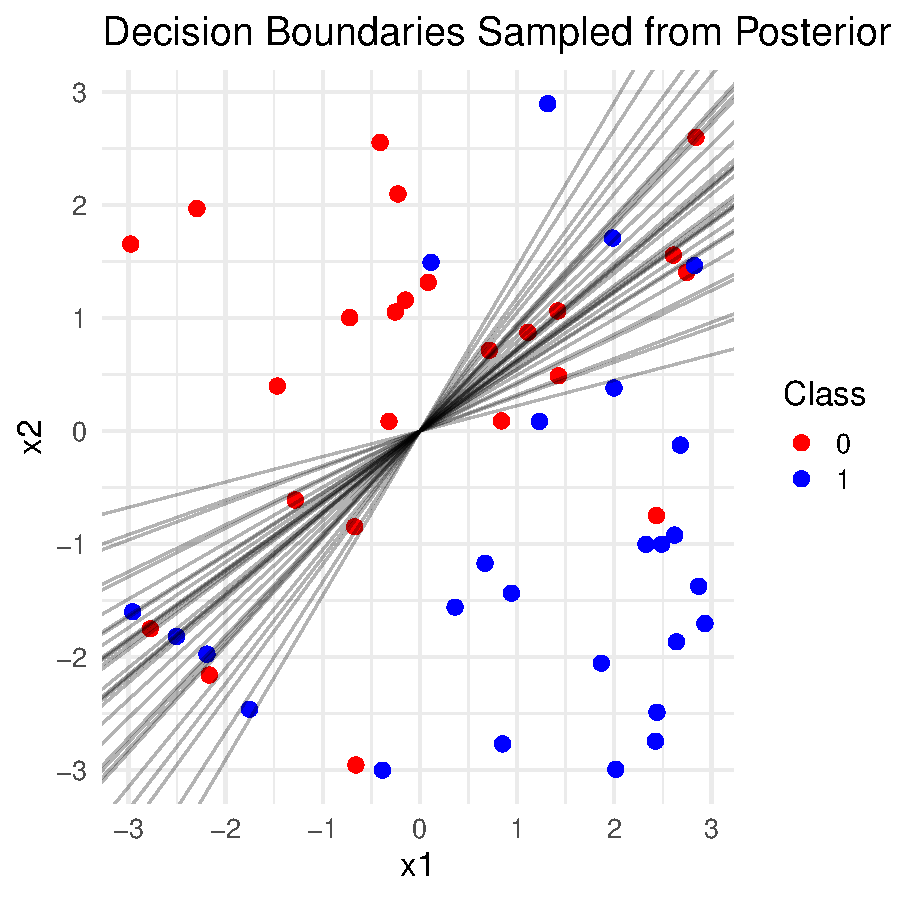
\includegraphics[width=0.7\textwidth]{mcmc.pdf}
    \caption{Decision boundaries drawn from 30 MCMC posterior samples of \(\theta = (w_1, w_2)\).}
  \end{figure}
\end{frame}

\section{Conclusion}

\begin{frame}{Conclusion}
\end{frame}


\end{document}
